\documentclass[aspectratio=169]{beamer}
\usepackage[utf8]{inputenc}
\usepackage{bookman}
\usetheme{Dresden}
\usepackage{graphicx}
\usepackage{hyperref}

\title[01-FDOC]{Welcome to MedTech Prototyping Skills!}
\author{Prototyping Skills (BME290L)}
\institute[Palmeri]{Mark L. Palmeri, M.D., Ph.D.}
\date{January 12, 2023}
\logo{
\includegraphics[width=0.1\textwidth]{BME-HorizontalLogo-Web-Blue.png}}

\begin{document}

\frame{\titlepage}

\frame{
    \frametitle{Outline}
    \tableofcontents
}

\section{Get to Know Each Other}
\subsection{Who am I?}
\frame{
    \frametitle{Long Duke track record...}
    \begin{itemize}
        \item Duke BME/ECE (1996--2000)
        \item Duke BME Grad (2005)
        \item Duke Med (2007)
    \end{itemize}
}

\frame{
    \frametitle{Teaching}
    \begin{itemize}
        \item BME153L/154L (Introduction to Circuit Analysis)
        \item BME354L (Introduction to Medical Instrumentation)
        \item BME547 (Medical Software Design)
        \item BME473L/474L (Medical Device Design)
        \item Founded BME Design Fellows program
        \item BME290L (MedTech Prototyping Skills)
    \end{itemize}
}

\frame{
    \frametitle{Research}
    \begin{itemize}
        \item Acoustic radiation force
        \item Ultrasonic elasticity imaging (non-invasive liver fibrosis, prostate cancer, MSK)
        \item Finite element method modeling
        \item Deep learning (signal and image processing) (POCUS)
        \item Medical devices for LMICs
        \item \url{https://palmeri.io}
    \end{itemize}
}

\frame{
    \frametitle{Fun}

    \begin{center}
        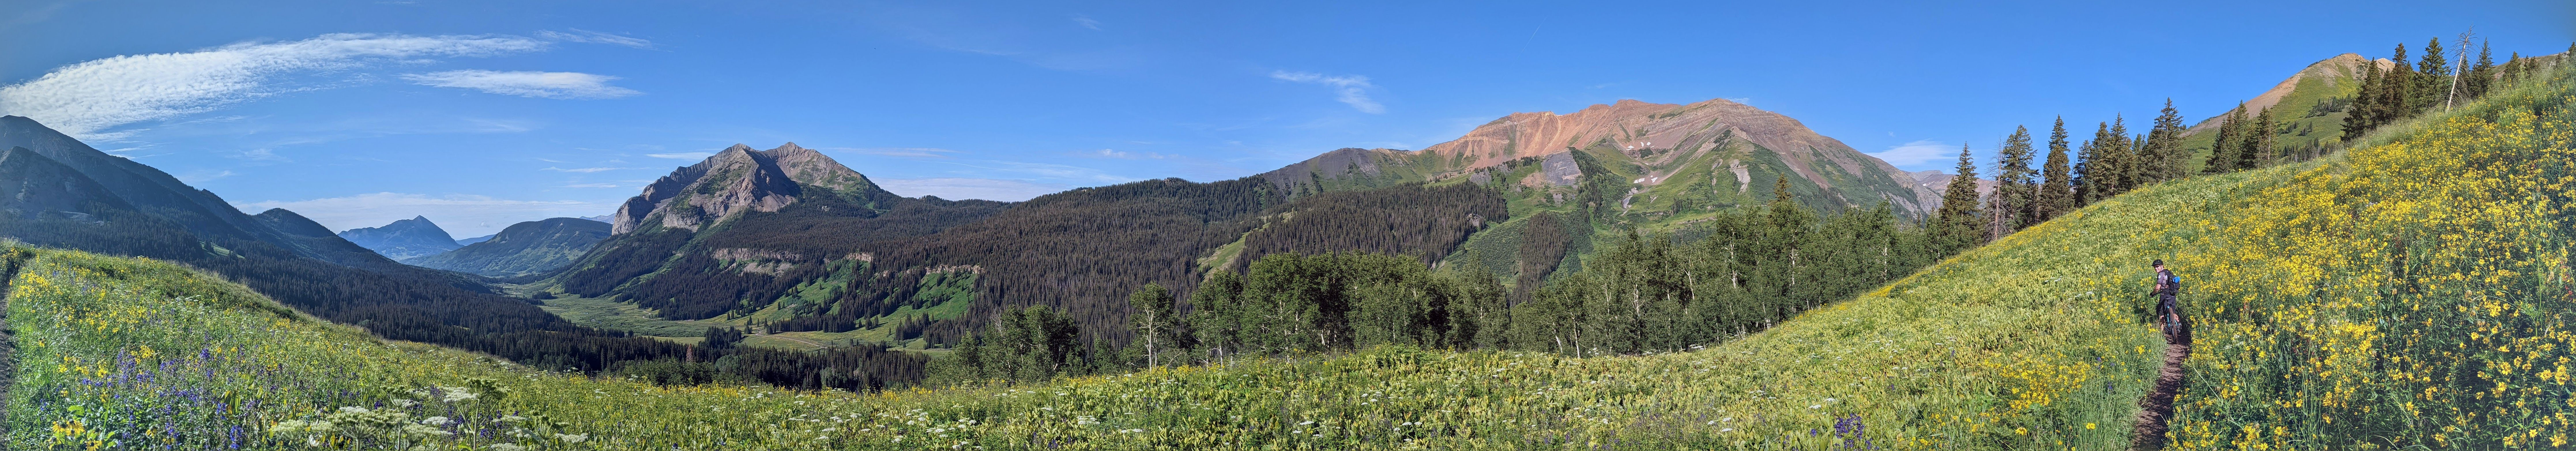
\includegraphics[width=1.0\textwidth]{CB_401.jpg}
    \end{center}
}

\subsection{Who are you?}
\frame{
    \frametitle{Who are you?}
    \begin{itemize}
        \item Name
        \item Hometown
        \item What do you aspire to do after Duke?
        \item Passion / memorable fact
    \end{itemize}
}

\section{Prototyping Skills}

\begin{frame}
    \frametitle{Why skills?}
    \begin{itemize}
        \item Do not want design ideas to be limited by what you ``think'' you can actually make!
        \item As the engineer, you bring both solution creativity and execution to the table.
        \item Most of the engineering curriculum has been ``book heavy'' to date.
        \begin{itemize}
            \item Functional Decomposition
            \item CAD/EDA (simulation, PCB layout)
            \item Fabrication \& Integration (3D printing, soldering, fastening, mounting)
            \item Verification \& Validation: testing to specifications 
            \item MCU Firmware Development (C, \texttt{git})
        \end{itemize}
    \end{itemize}
\end{frame}

\subsection{Functional Decomposition}

\begin{frame}
    \frametitle{FDA V\&V Waterfall}

    \begin{center}
        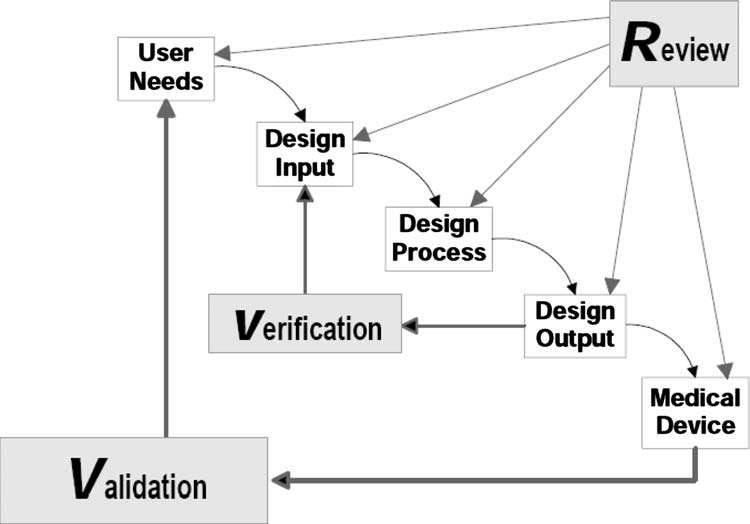
\includegraphics[width=0.5\textwidth]{DesignProcessWaterfall.jpg}
    \end{center}
    

\end{frame}

\begin{frame}
    \frametitle{Functional Decomposition}
    \begin{center}
        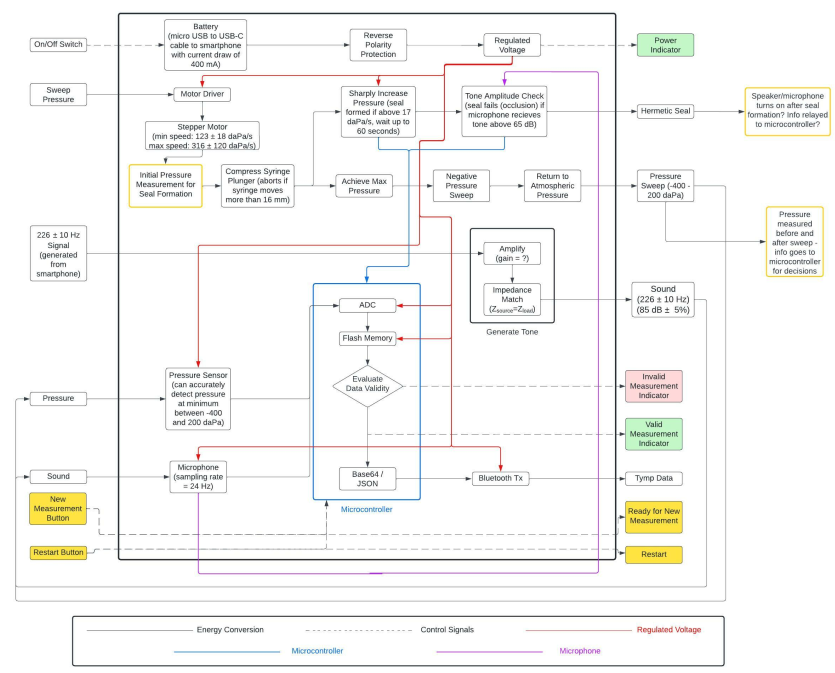
\includegraphics[width=0.5\textwidth]{func_decomp.png}
    \end{center}
\end{frame}

\begin{frame}
    \frametitle{User Action Flowchart}

   \begin{center}
        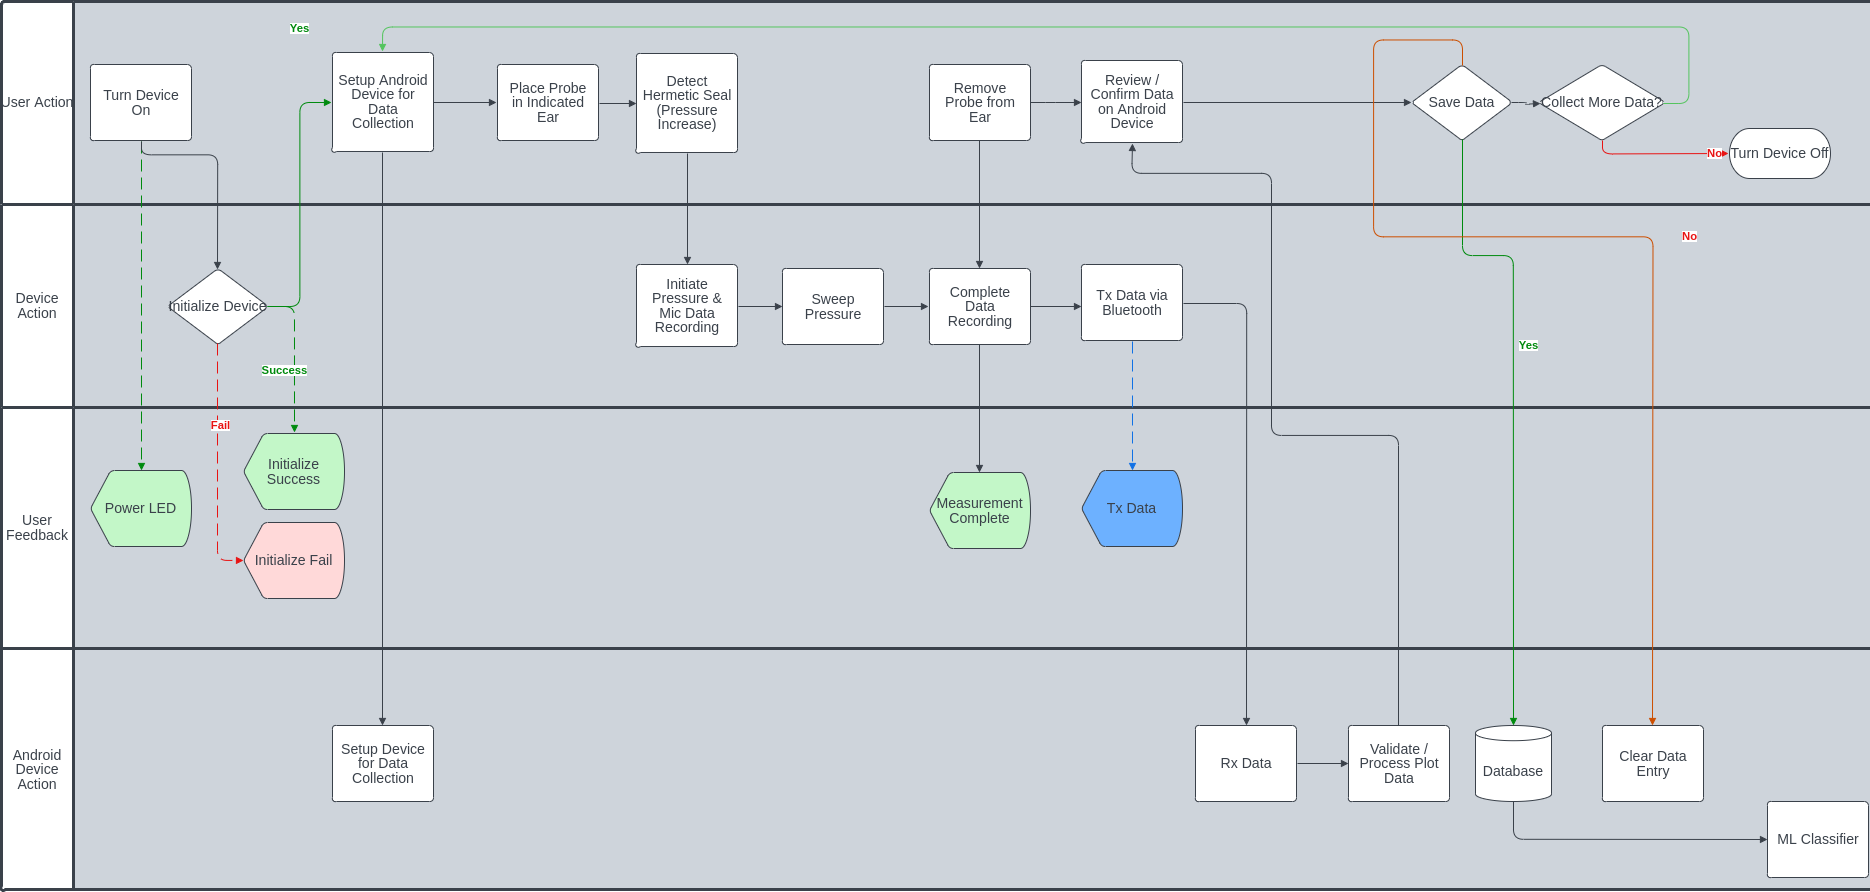
\includegraphics[width=0.8\textwidth]{user_action_flowchart.png}
   \end{center} 

\end{frame}

\subsection{CAD}
\frame{
    \frametitle{CAD: Competer Aided Design}
    Why CAD?
    \begin{itemize}
        \item Formally capture 2D projection sketches $\rightarrow$ 3D parts.
        \item Dimension consistency checks.
        \item Assemble multiple parts to check fit, interfaces and simulate stress/strain/movement.
        \item Translate to physical realization (e.g., 3D print, mil).
        \item General technical drawings for manufacturing.
        \item Capture design history, while facilitating iteration / change.
    \end{itemize}
}

\frame{
    \frametitle{onshape}

    \begin{center}
        
\includegraphics[width=0.33\textwidth]{logo-onshape-gray-green.png}
    \end{center}

    \begin{itemize}
        \item We will be using onshape, a cloud-based CAD package with a similar
        workflow to SolidWorks.
        \item You will be automatically registered to join Duke's onshape team
        (\url{https://duke.onshape.com}).
        \item Tutorials are available through \url{https:learn.onshape.com}
        (will be explicitly assigned).
    \end{itemize}
}

\begin{frame}
    \frametitle{mHealth Tympanometer}

    \begin{center}
        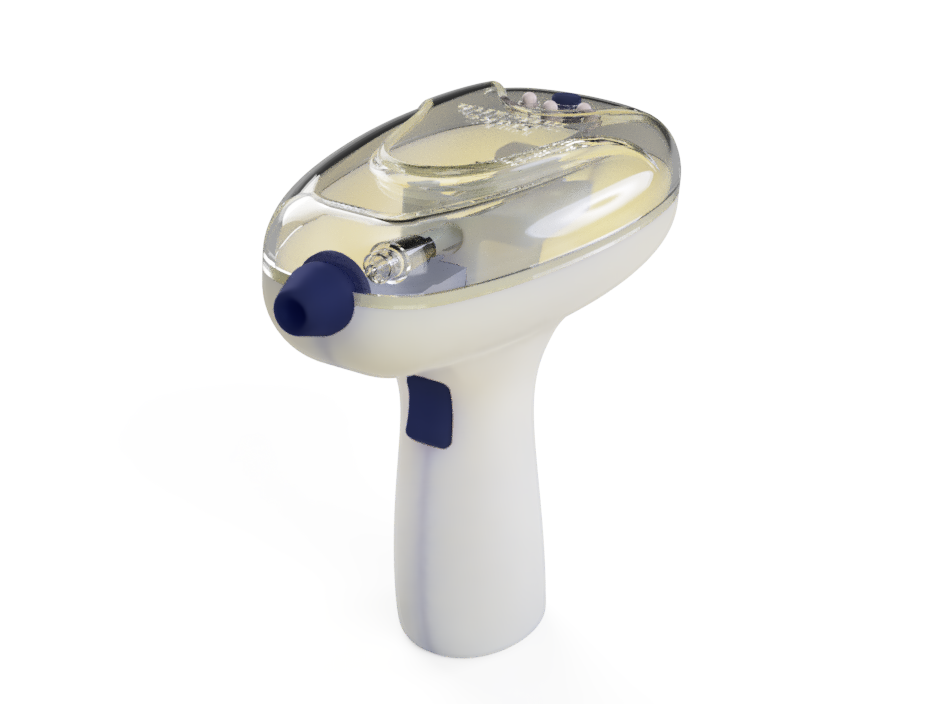
\includegraphics[width=0.55\textwidth]{rd2.png}
    \end{center}
\end{frame}

\subsection{EDA}
\frame{
    \frametitle{EDA: Electronics Design Automation}
    Why EDA?
    \begin{itemize}
        \item Formalize circuit schematics.
        \item Validate circuit behavior (design rules and SPICE simulations).
        \item Convert circuit to printed circuit board (more space efficient and permanent than a breadboard).
        \item Capture design history and facilitate rapid iteration.
        \item Generate 3D ``parts'' to integrate with CAD.
    \end{itemize}
}

\frame{
    \frametitle{KiCad}

    \begin{center}
        
\includegraphics[width=0.25\textwidth]{kicad_logo_small.png}
    \end{center}

    \begin{itemize}
        \item \url{https://kicad.org}
        \item A completely open-source alternative to Eagle.
        \item Just as capable as Altium Designer (to a point).
    \end{itemize}
}

\begin{frame}
    \frametitle{Schematic Capture}
    \begin{center}
        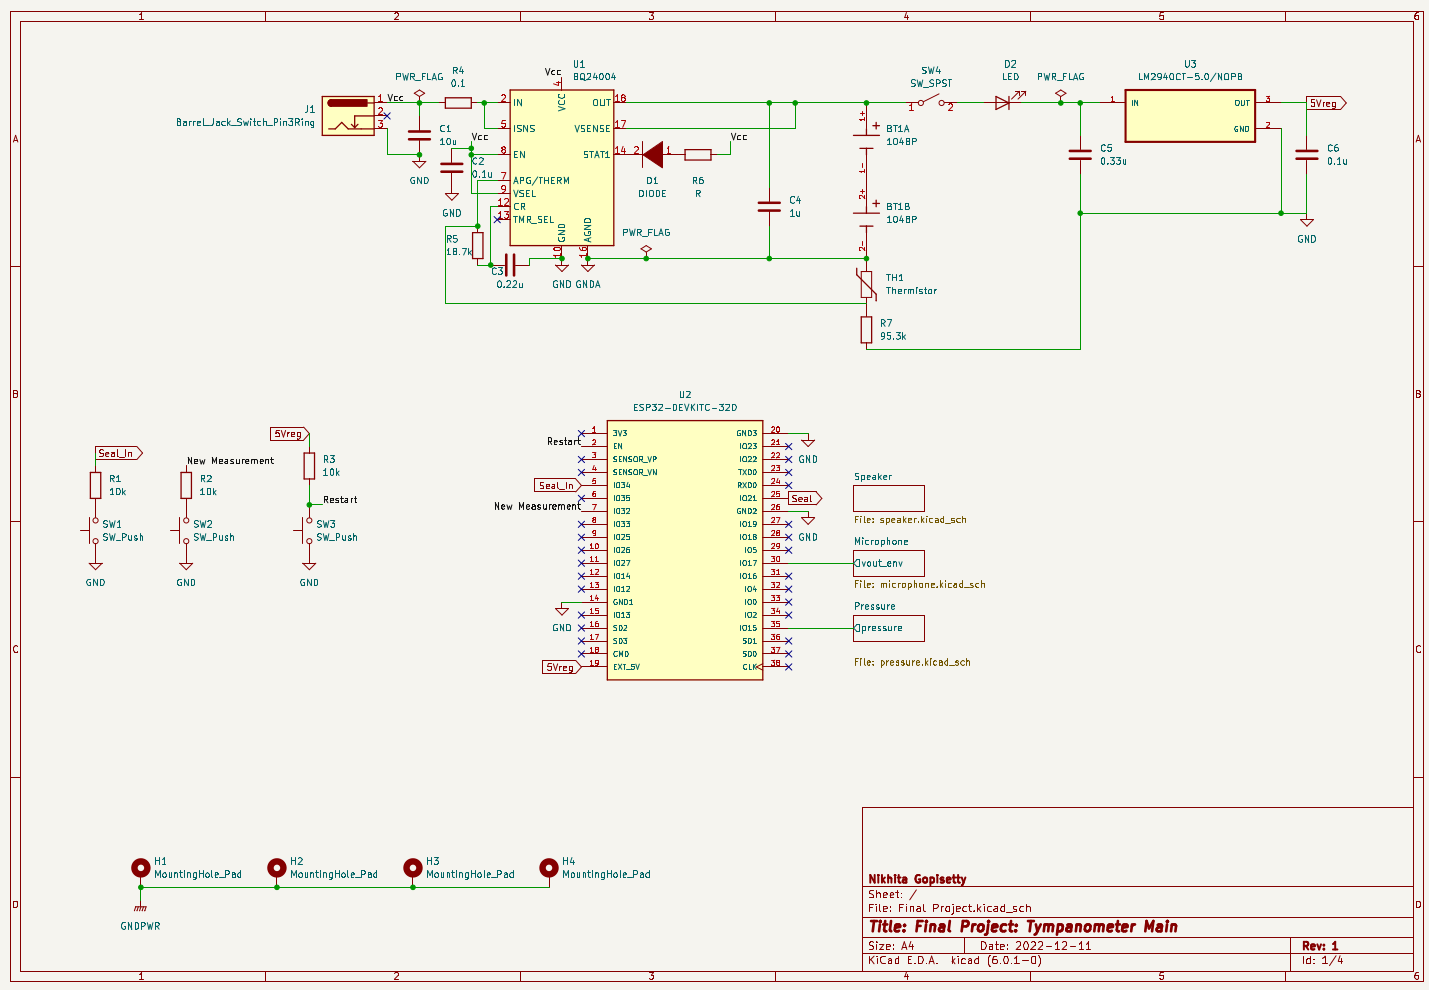
\includegraphics[width=0.6\textwidth]{schematic.png}
    \end{center}
\end{frame}


\begin{frame}
    \frametitle{PCB Layout}
    \begin{center}
        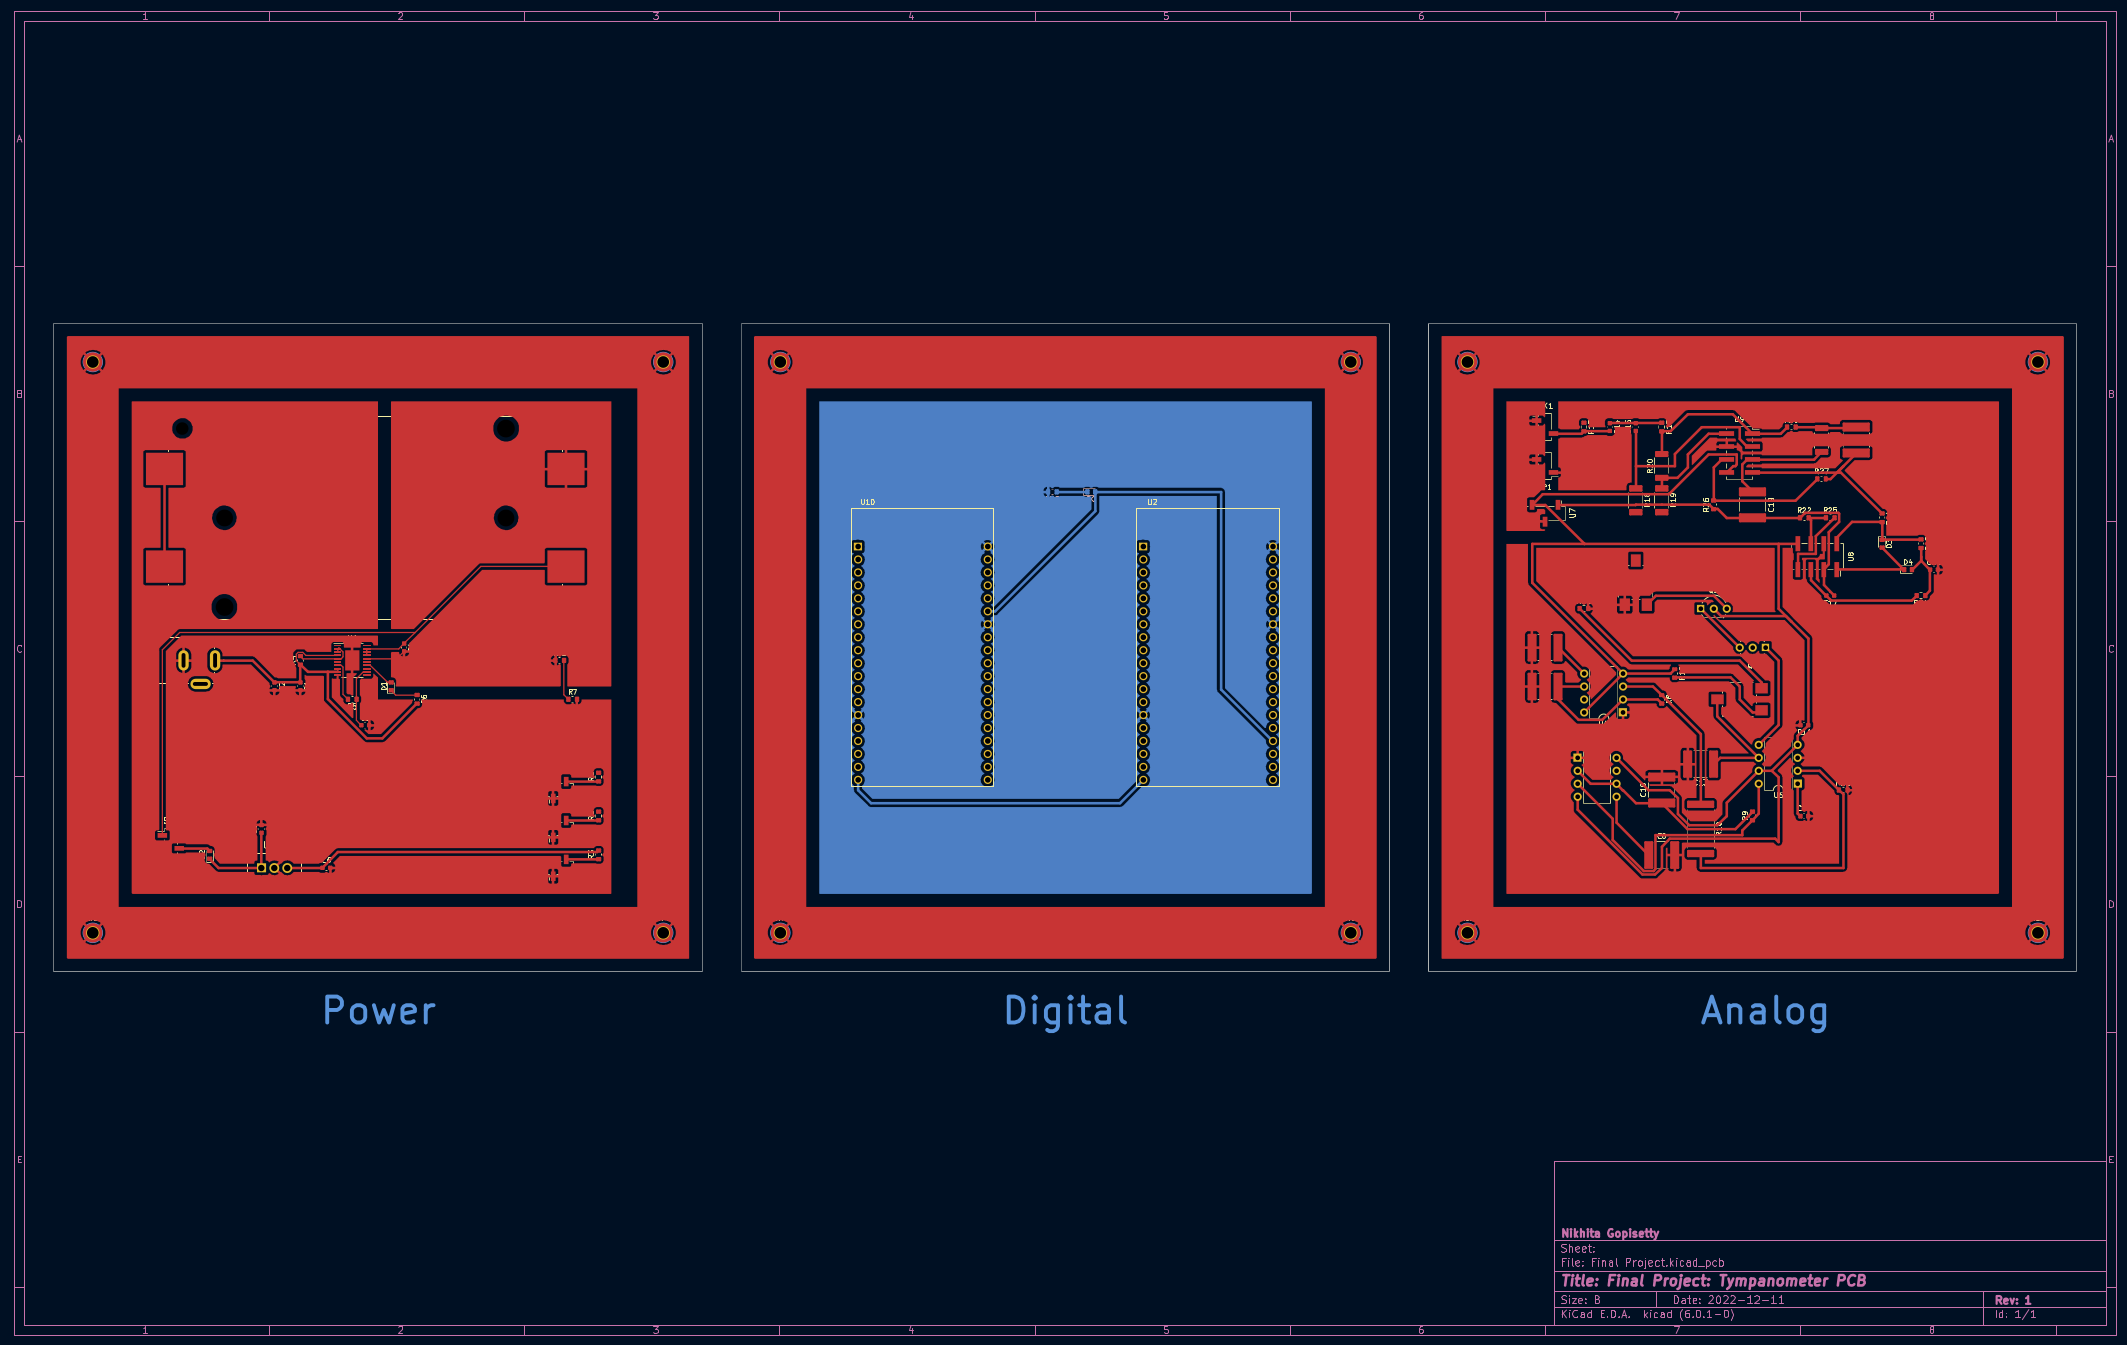
\includegraphics[width=0.6\textwidth]{pcb.png}
    \end{center}
\end{frame}

\begin{frame}
    \frametitle{PCB 3D Model}
    \begin{center}
        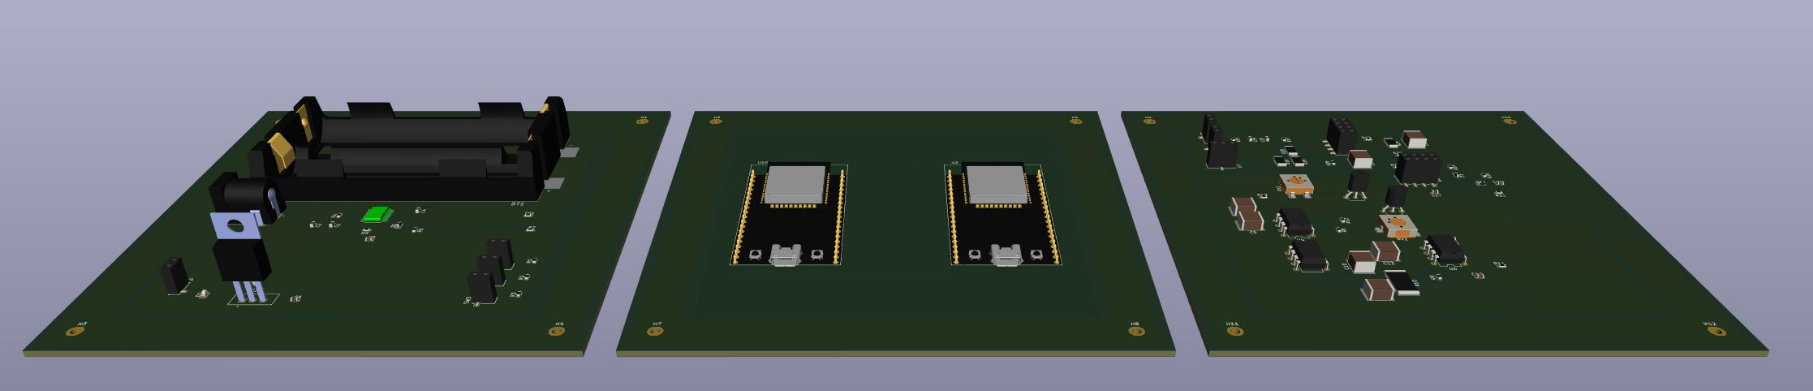
\includegraphics[width=0.9\textwidth]{pcb_step.png}
    \end{center}
\end{frame}

\section{Syllabus Review}
\frame{
    \frametitle{Syllabus}
    \begin{itemize}
        \item ``Live'' copy maintained on Sakai (will include revision number / compilation date)
        \item Many hyperlinks embedded in syllabus. 
        \item Lectures slides will be posted on Sakai before lecture.
        \item Assignments and lab exercises will be highlighted in lecture. 
        \item Detailed information, including due dates, posted on Gradescope.
    \end{itemize}
}

\section{Resumes / Portfolios}
\subsection{Resumes}
\frame{
    \frametitle{Resumes - make them more appealing and memorable}
    \begin{center}
        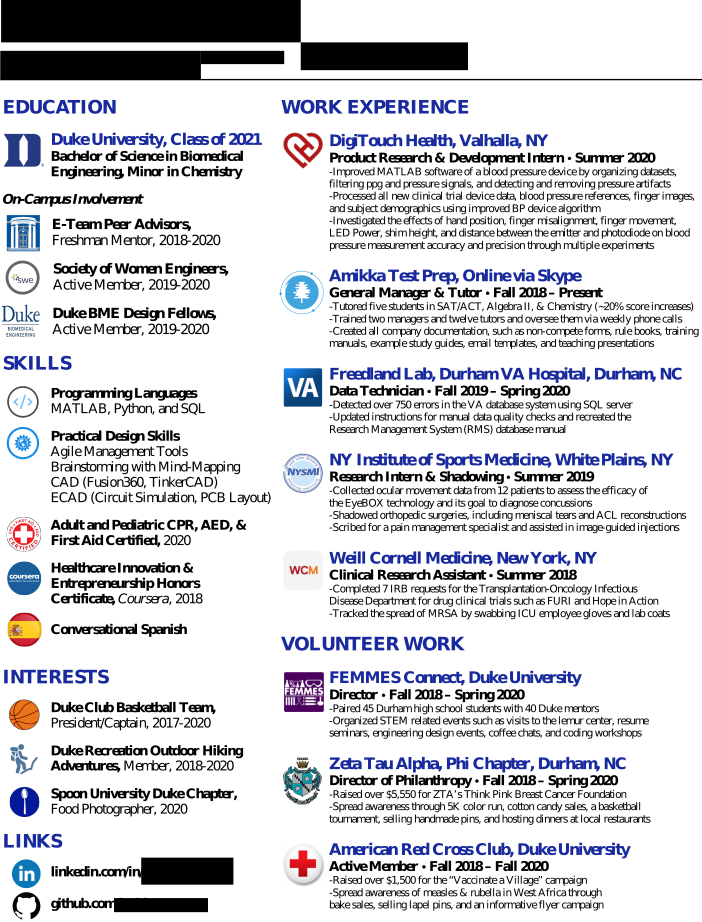
\includegraphics[width=0.3\textwidth]{JackieContento_Resume2020.png}
    \end{center}
   
}

\subsection{Online Portfolios}
\frame{
    \frametitle{Online Portfolio}
    \begin{itemize}
        \item Including links to online work product is great (e.g., \url{https://github.com/mlp6}).
        \item Showcasing your work is even better (e.g., \url{https://suyashkumar.com/}).
        \item Something to work on as you look to ``sell'' yourself for applying for internships, etc.
    \end{itemize}

}

\section{Lab}
\begin{frame}
    \frametitle{Lab This Week}

    \begin{itemize}
        \item Consider registering for the Friday morning session!
        \item Start at 14:00 (no food/drink in POD)
        \item Install software on personal laptops
        \item Confirm function
        \begin{itemize}
            \item Setup git to clone \& push
            \item Load KiCad project
            \item Log into Onshape
        \end{itemize}
        \item Order MCU
    \end{itemize}
\end{frame}


\end{document}
